\section{Introduction}
\label{sec:introduction}

% state the learning objective 
The laboratory assignment presented has of its purpose the study of a circuit
structured in four elementary meshes, through which exist seven resistors $R_i$,
a voltage source $V_a$, a current controlled voltage source $V_c$, a current
source $I_d$ and a voltage controlled current source $I_b$. The circuit can
be seen in Figure-\ref{fig:circuit}.

\lipsum[1-1]

Throughout the report it is presented a theoretical analysis, using both mesh
and nods methods, in Section~\ref{sec:analysis}; an analysis of the circuit,
in Section~\ref{sec:simulation}; a comparison of the results from both sections
Section~\ref{sec:analysis} and Section~\ref{sec:simulation}, in Section~\ref{sec:analysis};
and conclusions of the study, in Section~\ref{sec:conclusion}.


\begin{figure}[h] \centering
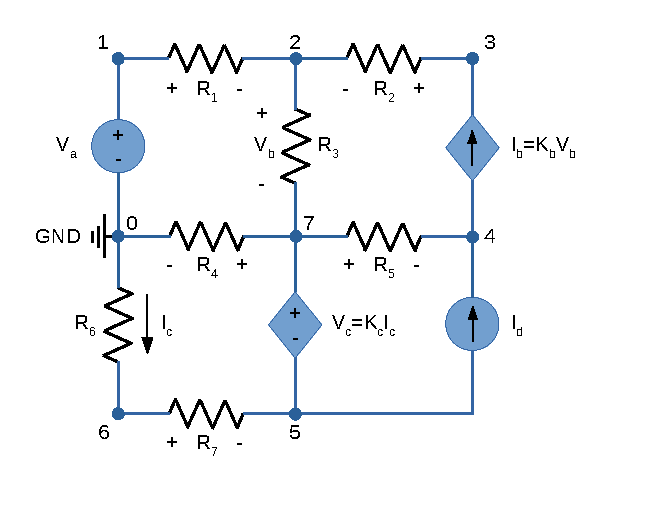
\includegraphics[width=0.4\linewidth]{circuit.pdf}
\caption{Voltage driven serial RC circuit.}
\label{fig:circuit}
\end{figure}

